\documentclass[11pt,a4paper]{article}
\usepackage[utf8]{inputenc}
\usepackage{amsmath}
\usepackage{amsfonts}
\usepackage{graphicx}

\usepackage[table,xcdraw]{xcolor}

\usepackage{caption}
\usepackage{subcaption}
\usepackage{float} % para que floten las imagenes o algo asi...
\usepackage{wallpaper} %paquete para usar una imagen como encabezado!
\usepackage{hyperref} %para usar hypervinculos 
\usepackage[export]{adjustbox} %para usar marcos en imagenes
\usepackage{eurosym} % para el euro
\usepackage{transparent} %para las marcas de agua
\usepackage{eso-pic}  %para las marcas de agua
\definecolor{azul_marcos}{RGB}{0,128,159} %defino el color azul de los marcos
\usepackage{sectsty} %esto es para cambiar el color de las fuentes creo
\renewcommand{\familydefault}{\sfdefault} % cambiamos la fuente a una sans
\sectionfont{\color{azul_marcos}}  % sets colour of sections
\subsectionfont{\color{azul_marcos}}  % sets colour of sections
\usepackage{pdfpages} %para insertar pdfs
\usepackage{amssymb}
\usepackage{pstcol} % para color
\usepackage{pst-node} % para diagramas
\usepackage{pst-plot} % para representacion de dat
\usepackage[spanish]{babel}
\addto\captionsspanish{\renewcommand\chaptername{Bloque}}
%\usepackage[total={18cm,21cm},top=2cm, left=2cm]{geometry}
\usepackage{anysize}
\pagestyle{plain}
%\markboth{left head}{right head}
%\markright{Guía de impresión FlexiSMART}
\marginsize{3cm}{2cm}{2.5cm}{1cm}
\title{Guida di Stampa di FlexiSMART}
\date{}

%configuracion de la marca de agua
\AddToShipoutPicture{
    \put(0,0){
        \parbox[b][\paperheight]{\paperwidth}{%
            \vfill
            \centering
            {\transparent{0.2}
\includegraphics[scale=1.25]{FOTOS/logofff}}%
            \vfill
        }
    }
}

\begin{document}
\ULCornerWallPaper{1}{FOTOS/header}
\LLCornerWallPaper{1}{FOTOS/footer}
%\maketitle
%\tableofcontents

\includepdf{PDF/DE_PORTADA.pdf}
\section{Che cos'è FlexiSMART?}lexiSMART è un filamento per stampa 3D FFF/FDM realizzato a partire da polimeri elastomeri termoplastici (TPE) con additivi chimici per renderlo più facile da stampare per la maggior parte delle stampanti 3D disponibili sul mercato.
\\\\
FlexiSMART è flessibile e riprende la sua forma dopo essere stato piegato, schiacciato o teso.

\section{Perchè usare FlexiSMART?}
FlexiSMART ti permette di conoscere un nuovo mondo di possibilità, grazie alla natura flessibile del suo filamento. Da oggi puoi stampare oggetti che prima, con un filamento rigido, non potevi stampare: Cover per  smartphones, tablets, scarpe, solette, ruote per auto radiocomandate, protesi, silent blocks, ingranaggi che necessitino di una certa adattabilità e, in generale, qualsiasi oggetto che ti venga in mente e che possa usufruire delle proprietà del filamento.
\\\\
FlexiSMART è stato progettato in modo da essere facile da stampare:
\begin{itemize}
\item Mantiene una certa rigidità in modo da poter essere stampato dalla maggior parte degli estrusori diretti, facendo nessuna o poche modifiche.
\item L'aderenza è eccellente. Può essere stampato anche senza piastra riscaldata.
\item La resistenza è molto elevata, per tanto i pezzi stampati non si deterioreranno rapidamente.
\item E il filamento flessibile con i prezzi migliori in tutta Europa.
\end{itemize}

\section{Dati tecnici e parametri di stampa}

\begin{table}[H]
\centering
\caption*{Dati tecnici}
\begin{tabular}{|
>{\columncolor[HTML]{FFFFFF}}l |
>{\columncolor[HTML]{FFFFFF}}c |}
\hline
\multicolumn{1}{|c|}{\cellcolor[HTML]{FFFFFF}\textbf{Materiale}}   & FlexiSMART (TPE)   \\ \hline
\textbf{Colori disponibili}              & 11                 \\ \hline
\textbf{Formati disponibili}             & 1kg, 250gr         \\ \hline
\textbf{Temperatura di deflessione termica} & 90ºC               \\ \hline
\textbf{Temperatura di fusione}            & 160ºC              \\ \hline
\textbf{Temperatura di decomposizione}    & \textgreater 240ºC \\ \hline
\textbf{Densità}                         & 0.96 gr / cm3      \\ \hline
\textbf{Stiramento massimo}              & 600\%              \\ \hline
\end{tabular}
\end{table}
\begin{table}[H]
\centering
\caption*{Parametri di stampa consigliati utilizzando un nozzle di 0.4 mm}
\begin{tabular}{|
>{\columncolor[HTML]{FFFFFF}}l |
>{\columncolor[HTML]{FFFFFF}}c |}
\hline
\multicolumn{1}{|c|}{\cellcolor[HTML]{FFFFFF}\textbf{Temperatura di stampa consigliata}} & 195º-220º              \\ \hline
\textbf{Velocità di stampa consigliata}                         & 20-60mm/s              \\ \hline
\textbf{Temperatura della piastra riscaldata}                                  & \textgreater 18º (Non necessita di piastra riscaldata)        \\ \hline
\textbf{Altezza ottimale dello strato}                                      & 0.2 mm                 \\ \hline
\textbf{Perimetri}                                                 & 3                      \\ \hline
\textbf{Top solid layers}                                           & 5                      \\ \hline
\textbf{Retrazione}                                                 & Disattivata o ridotta \\ \hline
\end{tabular}
\end{table}

Puoi scaricare i nostri profili di stampa completi per i principali programmi di laminazione  (Cura, Slic3r e SImplify3D) dalla nostra pagina web:
\\\\
\centerline{ {\huge \url{www.fffworld.com/documentation} } }
\\\\
I parametri ottimali dipenderanno dalla stampante 3D che utilizzi, ad ogni modo, questi sono dei buoni parametri che possono essere utilizzati come punto di partenza. Dopo poche stampe sarai in grado di determinare i limiti e la configurazione perfetta per la tua macchina.
\section{Problemi e soluzioni}
	\subsection{Problemi di estrusione con FlexiSMART}
La sfida principale quando si tratta di stampare con FlexiSMART e altri filamenti flessibili deriva dalla natura stessa del materiale che, essendo flessibile, non può essere spinto con la stessa facilità dei materiali rigidi, lo stesso principio per cui non si può spingere una corda.
\\\\
Il problema nasce quando ci sono laschi in certe parti dell'estrusore, in particolare, tra la drive-gear (la ruota dentata che spinge il filamento) e l'orifizio attraverso il quale il filamento accede all'hot-end (punta metallica che fonde il filamento).
\\\\
Quando questo spazio è sufficientemente grande, il filamento tende a uscire dal suo percorso e a formare un nodo che finisce per spuntare da un lato dell'estrusore, come si può vedere nell'immagine. 
\begin{figure}[H]
\centering
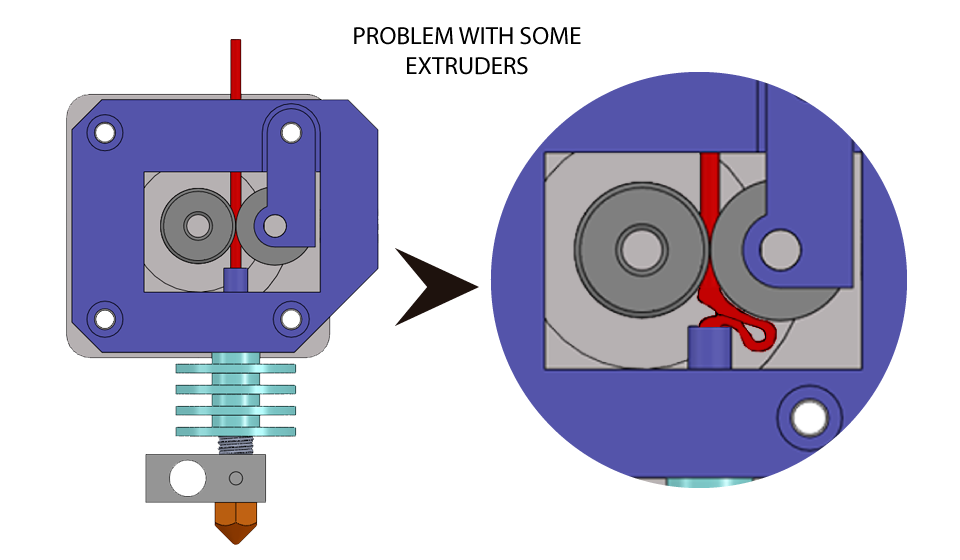
\includegraphics[width=0.5\textwidth,cfbox=azul_marcos 4pt 0pt]{FOTOS/NUDOS1}
\caption*{NON-optimized extruder for printing flexible filaments}
\end{figure}
Questo problema è di maggior portata se si utilizza un filamento da 1.75 mm dato che, avendo una sezione minore, è addirittura più propenso a uscire dal percorso..
\\\\
La velocità di estrusione è determinante affinché si verifichi questo problema. Se l'estrusore prova a spingere il filamento a una velocità troppo alta, si crea una pressione verso l'alto che fa sì che il filamento esca dal suo percorso naturale. Perciò il consiglio generale è di iniziare a stampare a una velocità bassa o molto bassa, e andare ad aumentarla fino a trovare la velocità massima sopportata dal tuo estrusore. Anche la dimensione del nozzle contribuisce alla velocità massima sopportata dato che, più grande è, più materiale fuso potrà essere estruso per unità di tempo e, per tanto, maggiore sarà la velocità alla quale questo si può fare. 
\\\\
Gli estrusori progettati per l'utilizzo di filamenti flessibili minimizzano i laschi, impedendo che il filamento possa uscire e utilizzano un sistema di doppia drive-gear per incanalare con precisione il filamento ed evitare completamente il problema suddetto, così come permettono di aumentare la velocità di stampa.
\begin{figure}[H]
\centering
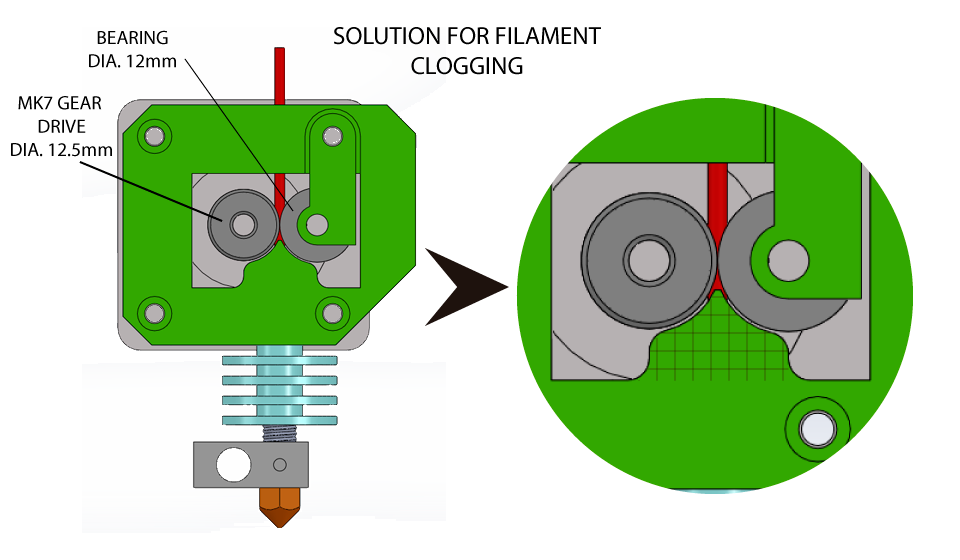
\includegraphics[width=0.5\textwidth,cfbox=azul_marcos 4pt 0pt]{FOTOS/NUDOS2}
\caption*{Optimized extruder for printing flexible filaments}
\end{figure}
\emph{FlexiSMART è stato progettato tenendo a mente questi problemi e ha una rigidità superiore rispetto ad altri filamenti flessibili, in modo che tali problemi possano essere minimizzati.}
\\\\
Ad ogni modo, su estrusori che non sono stati progettati per l'utilizzo di materiali elastici, possono comparire questi problemi.
	\subsection{Preparare l'estrusore per stampare FlexiSMART}Se stai sperimentando uno dei problemi sopra menzionati probabilmente dovrai adattare o sostituire il tuo estrusore. Esistono diverse opzioni che elenchiamo dettagliatamente di seguito.
		\subsubsection{Modificare il tuo estrusore}
A volte è possibile utilizzare FlexiSMART con estrusori non ottimizzati, realizzando alcune modifiche sull'estrusore stesso.
\\\\
Se stai sperimentando dei problemi nella stampa di FlexiSMART ti consigliamo di seguire i seguenti consigli, esposti in ordine di complessità.
			\paragraph{Limare il condotto in modo che il filamento acceda all'hot-end}\mbox{}\\\\
Se utilizzi un estrusore con il corpo di plastica, come gli estrusori stampabili, ti consigliamo di provare quanto segue. 
\\\\
Lima leggermente i bordi dell'orifizio che si trova proprio sotto del drive-gear, orifizio attraverso il quale viene incanalato il filamento verso l'hot-end. Questo permette di evitare sfregamenti e agganciamenti che possono causare i nodi sopra descritti.
\\\\
Può essere necessario smontare parte dell'estrusore per effettuare questa operazione.
			\paragraph{Inserire un tubo di teflon nell'estrusore}\mbox{}\\\\
Una seconda opzione, più complicata ma più efficace, consiste nell'inserire un tubo di teflon (PTFE) nell'orifizio menzionato. Questa tecnica permette inoltre di ridurre lo spazio con la drive-gear, dato che il tubo in questione può essere collocato molto vicino alla drive-gear. Si può anche modificare l'entrata del tubo di teflon per adattarlo alla forma del drive-gear, lasciando uno spazio minimo.
\\\\
In generale questa tecnica presuppone la trapanatura dell'estrusore per permettere l'inserimento del tubo di teflon. Di seguito potete vedere un'immagine del risultato:
\begin{figure}[H]
    \centering
    \begin{subfigure}[b]{0.3\textwidth}
        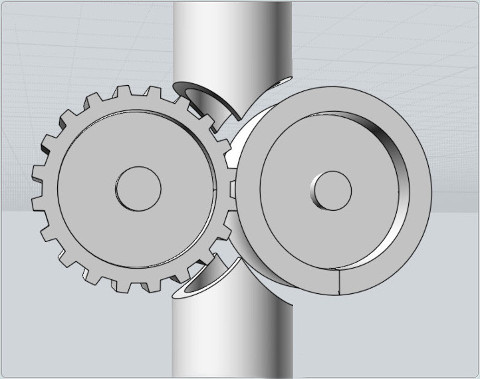
\includegraphics[width=\textwidth,cfbox=azul_marcos 4pt 0pt]{FOTOS/TEFLON1}
    \end{subfigure}
    ~ %add desired spacing between images, e. g. ~, \quad, \qquad, \hfill etc. 
      %(or a blank line to force the subfigure onto a new line)
    \begin{subfigure}[b]{0.3\textwidth}
        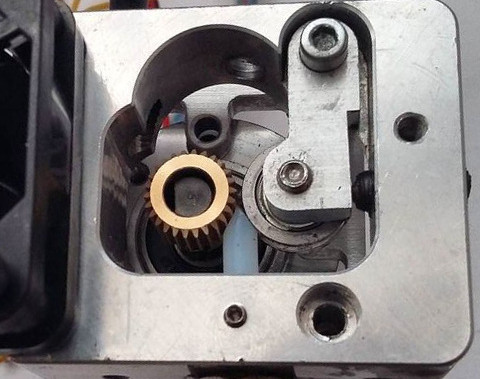
\includegraphics[width=\textwidth,cfbox=azul_marcos 4pt 0pt]{FOTOS/TEFLON2}
    \end{subfigure}
    ~ %add desired spacing between images, e. g. ~, \quad, \qquad, \hfill etc. 
    %(or a blank line to force the subfigure onto a new line)
    \begin{subfigure}[b]{0.3\textwidth}
        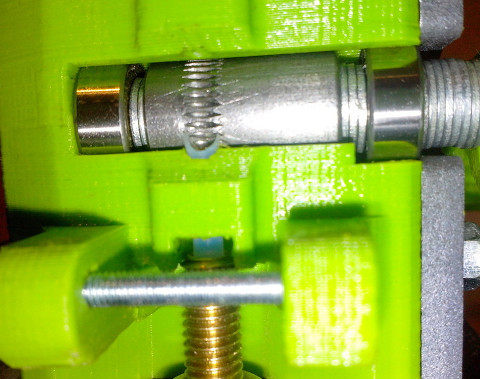
\includegraphics[width=\textwidth,cfbox=azul_marcos 4pt 0pt]{FOTOS/TEFLON3}
    \end{subfigure}
    \caption*{PTFE (Teflon) tube insertions}
\end{figure}
			\paragraph{Stampare una guida per il filamento e collocarla nell'estrusore }\mbox{}\\\\
La terza opzione consiste nello stampare un pezzo che faccia da guida per il filamento e collocarlo sotto il drive-gear. Questi pezzi solitamente hanno una forma triangolare e devono essere progettati rispettando le dimensioni di ogni estrusore. 
\\\\
In Internet, in siti come \url{www.thingiverse.com}, si possono scaricare questo tipo di adattatori per alcuni degli estrusori più comuni. Ad ogni modo, si tratta di un disegno semplice, che quanti possiedono conoscenze di disegno 3D potranno creare da zero con facilità.
\begin{figure}[H]
    \centering
    \begin{subfigure}[b]{0.5\textwidth}
        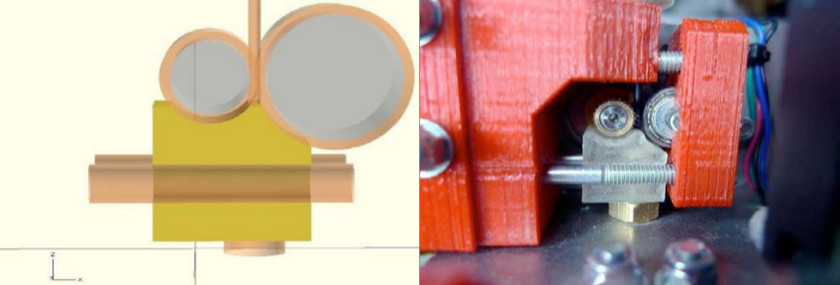
\includegraphics[width=\textwidth,cfbox=azul_marcos 4pt 0pt]{FOTOS/GUIA1}
    \end{subfigure}
    ~ %add desired spacing between images, e. g. ~, \quad, \qquad, \hfill etc. 
      %(or a blank line to force the subfigure onto a new line)
    \begin{subfigure}[b]{0.5\textwidth}
        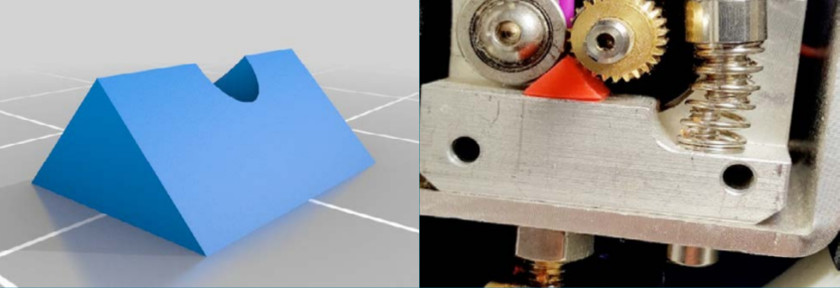
\includegraphics[width=\textwidth,cfbox=azul_marcos 4pt 0pt]{FOTOS/GUIA2}
    \end{subfigure}
    ~ %add desired spacing between images, e. g. ~, \quad, \qquad, \hfill etc. 
    %(or a blank line to force the subfigure onto a new line)
    \begin{subfigure}[b]{0.5\textwidth}
        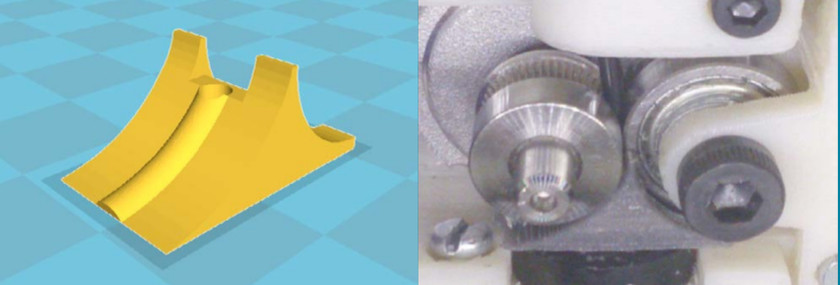
\includegraphics[width=\textwidth,cfbox=azul_marcos 4pt 0pt]{FOTOS/GUIA3}
    \end{subfigure}
    \caption*{Printable filament guides}
\end{figure}	

	\paragraph{Regolare la pressione del drive-gear sopra il filamento}\mbox{}\\\\
Considerato che si tratta di un materiale flessibile, è particolarmente importante che la pressione del meccanismo che spinge il filamento verso l'hot-end non sia eccessiva. Nei filamenti rigidi un eccesso di pressione produrrà piccole tacche nella superficie, ma nel caso di FlexiSMART una pressione eccessiva deformerà la sezione del filamento, dandogli una forma ovale che fa sì che questo sia più propenso a otturare l'estrusore.
\\\\
Gli estrusori progettati per la stampa di filamenti flessibili tengono in considerazione queste eventualità e sono provvisti di un meccanismo per regolare la pressione del meccanismo motore. Se il tuo estrusore permette di regolare detta pressione ti consigliamo di regolarla quando utilizzi FlexiSMART. La pressione adeguata sarà la minima necessaria affinché l'estrusore possa muovere il filamento.
\\\\
Se il tuo estrusore non dispone del meccanismo per regolare la pressione, puoi comunque ridurla cambiando la molla o riducendo il percorso possibile con la collocazione di un cuneo nel punto preciso. Come esempio ti mostriamo un'immagine di come ridurre la pressione in un estrusore che non è predisposto per questo:
\begin{figure}[H]
\centering
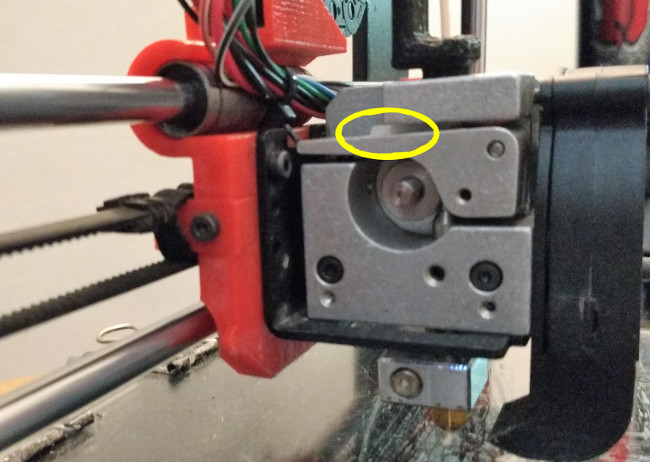
\includegraphics[width=0.5\textwidth,cfbox=azul_marcos 4pt 0pt]{FOTOS/SOLUCION1}
\caption*{HeatCore Extruder. BQ Hephestos and BQ Witbox}
\end{figure}
			\paragraph{Aggiungere tensione tra la bobina e l'estrusore}\mbox{}\\\\
Si è notato che in alcuni modelli di stampante è bene che, quando si utilizza un filamento flessibile, ci sia una tensione tra la bobina e l'estrusore in modo che il filamento non rimanga appeso. 
\\\\
Per ottenerla puoi provare a frenare la bobina, in modo che l'estrusore debba tirare leggermente il filamento per srotolarlo. Si può anche collocare un accessorio simile a quello in foto per ottenere lo stesso scopo.
\begin{figure}[H]
\centering
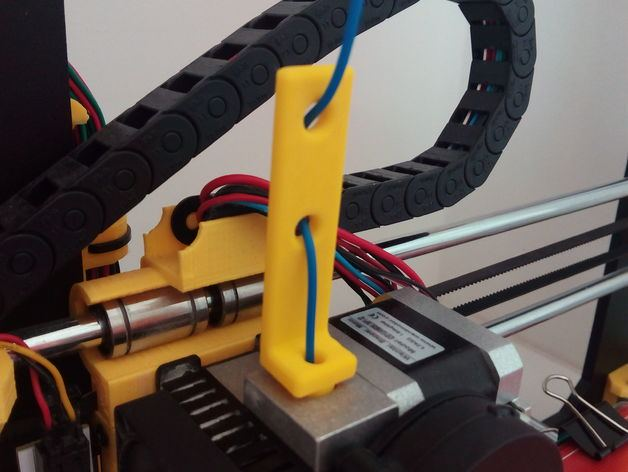
\includegraphics[width=0.5\textwidth,cfbox=azul_marcos 4pt 0pt]{FOTOS/SOLUCION2}
\caption*{Designed for BQ Unibody and BQ Hephestos extruder}
\end{figure}
		\subsubsection{Sostituire il tuo estrusore con uno ottimizzato}
Ad oggi i filamenti flessibili sono diventati tanto popolari che è difficile che una stampante di ultima generazione non sia preparata alla loro stampa.
\\\\
Inoltre, sono molti i progettisti che hanno creato estrusori stampabili capaci di stampare FlexiSMART e altri filamenti. Questi estrusori possono essere scaricati da pagine come Thingiverse, per essere stampati e assemblati a casa. 
\\\\
Inoltre sono sempre di più gli estrusori commerciali predisposti alla stampa di filamenti flessibili che possono essere acquistati ed essere montati nelle nostre stampanti. 
			\paragraph{Estrusori stampabili DIY}
\mbox{}\\\\
Alcuni di questi estrusori sono stati progettati da zero, altri sono modifiche realizzate su disegni già esistenti. Qui andiamo a presentare una lista non esaustiva di disegni di estrusori che possono essere scaricati da Internet. Seguendo ogni link potrai trovare la lista di componenti completa, così come istruzioni di montaggio e commenti di altri utenti. 
\\\\
L'hot-end che viene installato nell'estrusore deve avere un pezzo di teflon (PTFE) al suo interno per evitare frizioni, in modo che FlexiSMART si stampi correttamente. FlexiSMART è stato provato con successo nei seguenti hot-ends\footnote{Bisogna tenere conto del fatto che la prova è stata effettuata con hot-ends originali e non possiamo garantire lo stesso risultato con repliche di questi.}:
\begin{itemize}
\item J-Head MKV-B
\item Budassnozzle V1.3
\item E3D v6
\item Leonnozzle V2
\end{itemize}
A seconda della stampante che viene utilizzata, alcuni di questi estrusori saranno più facili da installare, dato che possono rimpiazzare direttamente l'estrusore originale della macchina.
\begin{figure}[H]
    \centering
    \begin{subfigure}[b]{0.4\textwidth}
        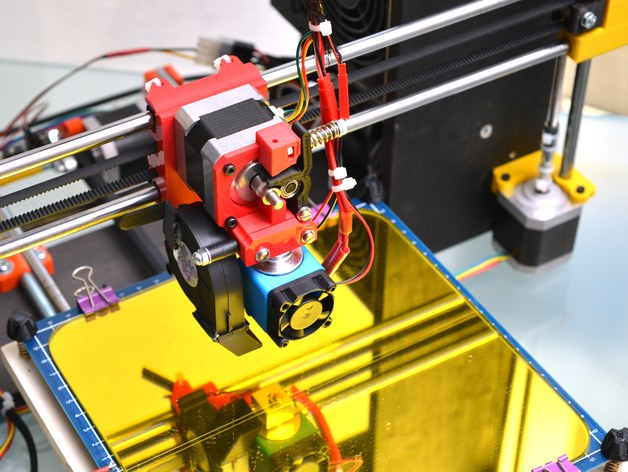
\includegraphics[width=\textwidth,cfbox=azul_marcos 4pt 0pt]{FOTOS/EXTRUSOR1}
		\caption*{\href{http://www.thingiverse.com/thing:147705}{{\footnotesize Direct-drive hinged extruder for E3D/J-Head hot-end (Prusa i3) by ffleury}}}
    \end{subfigure}
    ~ \qquad%add desired spacing between images, e. g. ~, \quad, \qquad, \hfill etc. 
      %(or a blank line to force the subfigure onto a new line)
    \begin{subfigure}[b]{0.4\textwidth}
        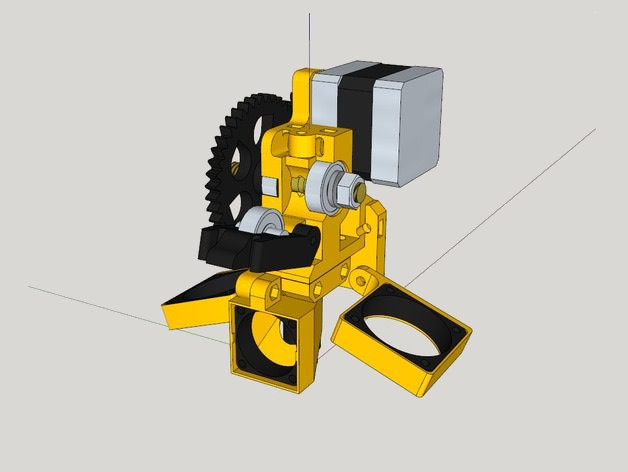
\includegraphics[width=\textwidth,cfbox=azul_marcos 4pt 0pt]{FOTOS/EXTRUSOR2}
		\caption*{\href{http://www.thingiverse.com/thing:512338}{{\footnotesize Wade L3K Extruder (prusa I3) compatible filament flexible By Skarab}}}
    \end{subfigure}
\end{figure}
\begin{figure}[H]
    \centering
    ~ %add desired spacing between images, e. g. ~, \quad, \qquad, \hfill etc. 
    %(or a blank line to force the subfigure onto a new line)
    \begin{subfigure}[b]{0.4\textwidth}
        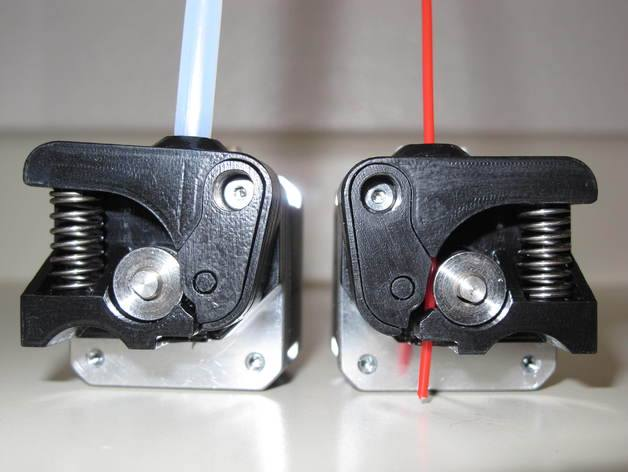
\includegraphics[width=\textwidth,cfbox=azul_marcos 4pt 0pt]{FOTOS/EXTRUSOR3}
		\caption*{\href{http://www.thingiverse.com/thing:403438}{{\footnotesize Printrbot Flexible Filament Direct Drive Extruder by thirdhorizon}}}
    \end{subfigure}
    ~ \qquad %add desired spacing between images, e. g. ~, \quad, \qquad, \hfill etc. 
    %(or a blank line to force the subfigure onto a new line)
    \begin{subfigure}[b]{0.4\textwidth}
        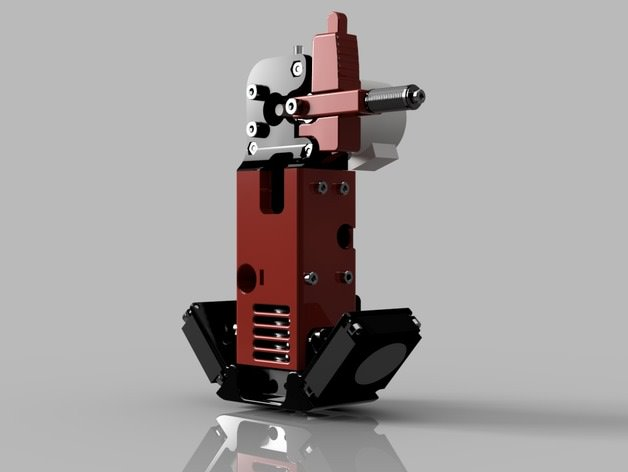
\includegraphics[width=\textwidth,cfbox=azul_marcos 4pt 0pt]{FOTOS/EXTRUSOR4}
		\caption*{\href{http://www.thingiverse.com/thing:1102900}{{\footnotesize Ultimaker 2 PG35L Direct Drive Extruder for 1.75mm E3D v6 Hotend by jasonatepaint}}}
    \end{subfigure}
\end{figure}
			\paragraph{Estrusori commerciali}\mbox{}\\\\
Acquistare un estrusore commerciale è più costoso che costruirne uno casalingo, tuttavia, di solito rendono meglio che questi ultimi e sono l'opzione migliore quando si utilizza il filamento flessibile in modo intensivo.
\\\\
Questi estrusori sono stati appositamente progettati per evitare tutti i problemi sopra menzionati e qualcuno di essi può estruire FlexiSMART a una velocità superiore ai 70 mm/s.
\begin{figure}[H]
    \centering
    \begin{subfigure}[b]{0.4\textwidth}
        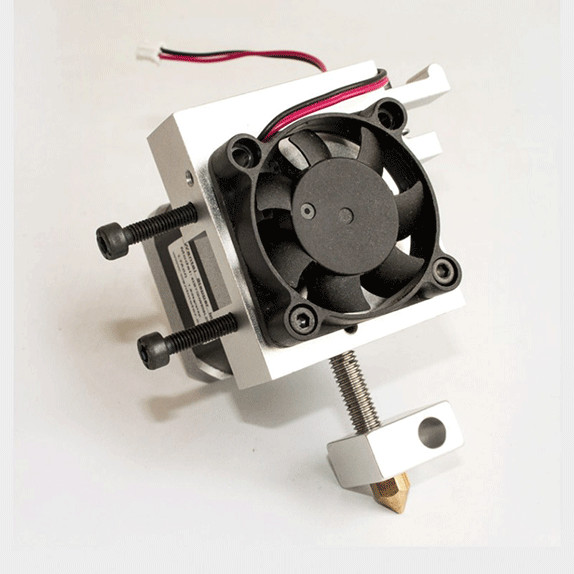
\includegraphics[width=\textwidth,cfbox=azul_marcos 4pt 0pt]{FOTOS/EXTRUSOR5}
		\caption*{\href{http://www.recreus.com}{{\footnotesize Recreus Extruder - Price aprox. 100\euro}}}
    \end{subfigure}
    ~ \qquad%add desired spacing between images, e. g. ~, \quad, \qquad, \hfill etc. 
      %(or a blank line to force the subfigure onto a new line)
    \begin{subfigure}[b]{0.4\textwidth}
        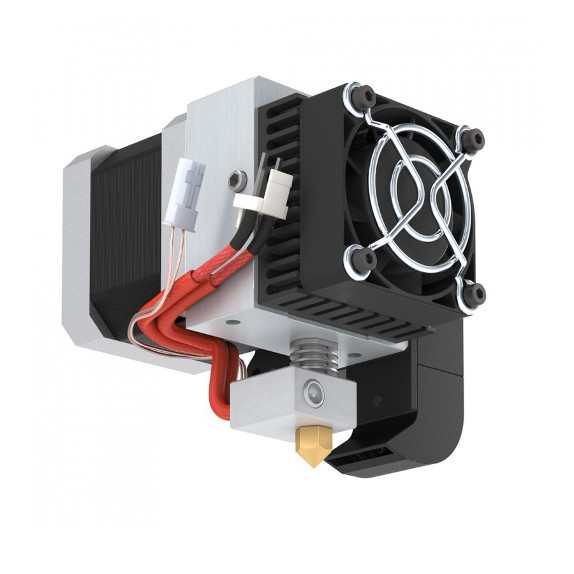
\includegraphics[width=\textwidth,cfbox=azul_marcos 4pt 0pt]{FOTOS/EXTRUSOR6}
		\caption*{\href{http://www.bq.es}{{\footnotesize BQ HeatCore DDG Extruder - Price 140\euro}}}
    \end{subfigure}
\end{figure}
\begin{figure}[H]
    \centering
    ~ %add desired spacing between images, e. g. ~, \quad, \qquad, \hfill etc. 
    %(or a blank line to force the subfigure onto a new line)
    \begin{subfigure}[b]{0.4\textwidth}
        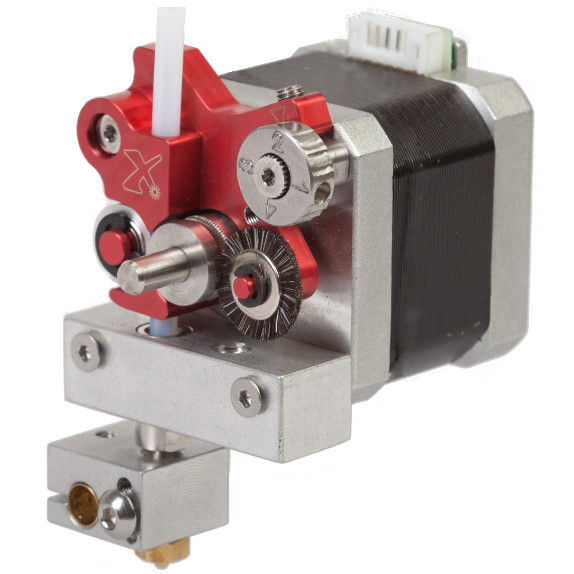
\includegraphics[width=\textwidth,cfbox=azul_marcos 4pt 0pt]{FOTOS/EXTRUSOR7}
		\caption*{\href{https://flexionextruder.com/}{{\footnotesize Flexion Extruder - Price aprox. 140\euro}}}
    \end{subfigure}
    ~ \qquad %add desired spacing between images, e. g. ~, \quad, \qquad, \hfill etc. 
    %(or a blank line to force the subfigure onto a new line)
    \begin{subfigure}[b]{0.4\textwidth}
        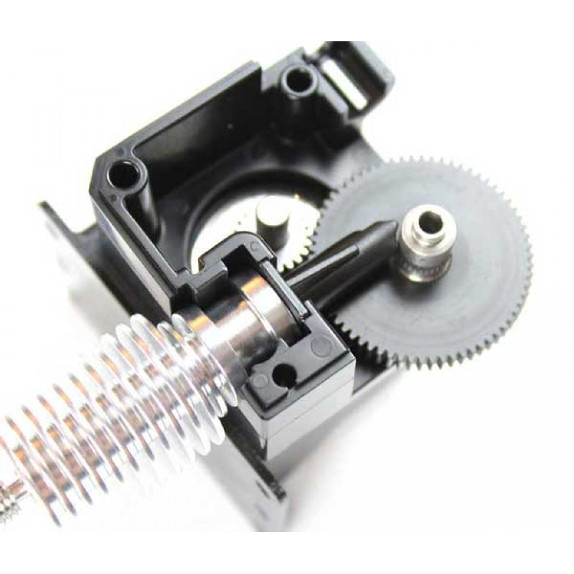
\includegraphics[width=\textwidth,cfbox=azul_marcos 4pt 0pt]{FOTOS/EXTRUSOR8}
		\caption*{\href{www.e3d-online.com}{{\footnotesize Titan Extruder - Price aprox. 70\euro}}}
    \end{subfigure}
\end{figure}
\section{Consigli per un uso ottimale di FlexiSMART}
	\subsection{La retrazione}
La retrazione è una tecnica usata nelle stampanti 3D FFF/FDM per migliorare la finitura dei pezzi. Consiste nel comandare all'estrusore che ritiri alcuni centimetri di filamento quando questo cambia di posizione, per evitare lo stringing o la comparsa di piccoli fili di filamento tra le diverse parti del pezzo che si sta stampando.
\begin{figure}[H]
\centering
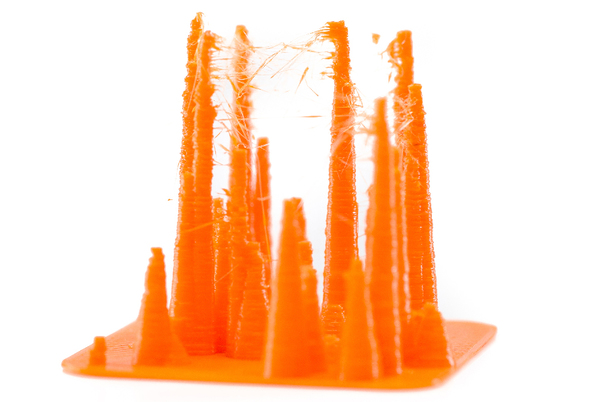
\includegraphics[width=0.5\textwidth,cfbox=azul_marcos 4pt 0pt]{FOTOS/RETRACCION1}
\caption*{A part with stringing problems}
\end{figure}
Quando si utilizzano filamenti flessibili può succedere che nel tentare una retrazione molto brusca il filamento si tenda invece di retrocedere. Perciò è caldamente consigliato utilizzare dei parametri di retrazione diversi da quelli usati con filamenti rigidi.
\\\\
I 2 parametri che possiamo controllare nella retrazione sono la dimensione, o quantità lineare in millimetri di filamento ritratto, e la velocità in mm/s dell'operazione. Entrambi i valori devono essere inferiori a quelli utilizzati abitualmente. Il modo ottimale per calibrare questi valori è effettuare delle prove per verificare quali sono i valori massimi che sopporta la tua stampante nella stampa con FlexiSMART. In ogni caso, come punto di partenza puoi usare i valori consigliati da noi:
\begin{description}
\item [Dimensioni di retrazione:] 1.5 mm
\item [Velocità di retrazione:] 40 mm/s
\end{description}
A seconda della stampante può essere che sia necessario disattivare totalmente la retrazione.
	\subsection{Stampa sequenziale}
Un filamento flessibile FlexiSMART presenta una viscosità differente a quella di altri materiali quando raggiunge la sua temperatura di fusione. Per questo è più propenso a lasciare piccoli fili di filamento tra diverse parti del pezzo quando il nozzle deve spostarsi da un punto ad un altro senza estruire. 
\begin{figure}[H]
\centering
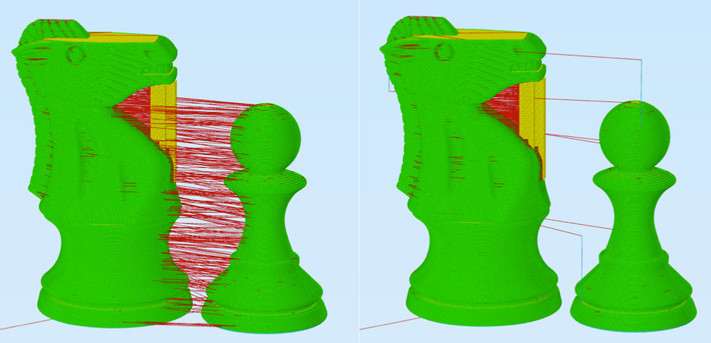
\includegraphics[width=0.5\textwidth,cfbox=azul_marcos 4pt 0pt]{FOTOS/SEQUENTIALPRINTING}
\caption*{Comparison between printing routes of simultaneus and sequential printing}
\end{figure}
Inoltre, quando si stampano diversi pezzi distinti allo stesso tempo, questi piccoli fili possono crearsi tra i pezzi, dato che il nozzle deve saltare da uno all'altro costantemente.
\\\\
Come già è stato detto precedentemente, questo effetto può essere ridotto utilizzando la retrazione, ma è inoltre caldamente consigliato che i distinti pezzi vengano stampati in modo sequenziale invece che simultaneo.
\\\\
Con la stampa sequenziale intendiamo la stampa completa di un pezzo prima di cominciare a stampare il seguente.
\\\\
Questo si può ottenere in 2 modi diversi:
\begin{itemize}
\item L'opzione più banale è di stampare solo un pezzo e, una volta terminato, ripetere la stessa stampa tante volte quante si desideri.
\item La seconda alternativa, più avanzata e che presenta alcuni limiti, è di utilizzare l'opzione offerta da alcuni programmi di laminazione di stampare un pezzo alla volta. La dimensione massima dei pezzi che possono essere stampati utilizzando questo metodo è data dalle dimensioni del nozzle e dalla disposizione degli assi della stampante. Consigliamo caldamente di informarsi su come utilizzare queste opzioni per non correre il rischio di danneggiare la stampante. Puoi farlo attraverso i link seguenti:
\end{itemize}
\url{https://www.simplify3d.com/support/tutorials/multi-part-printing/}\\
\url{http://manual.slic3r.org/advanced/sequential-printing}\\
\url{https://ultimaker.com/en/community/3843-force-cura-to-print-objects-separately}
	\subsection{Il primo strato}
Il primo strato è il fondamento del resto di strati è può determinare la differenza tra una stampa soddisfacente e una stampa mancata.
\\\\
Nella stampa con FlexiSMART si deve porre una particolare attenzione al primo strato dato che, a volte, una stampante livellata correttamente per stampare con PLA o ABS può non esserlo per stampare FlexiSMART in modo corretto.
\\\\
Per sapere se la stampante è livellata correttamente bisogna osservare attentamente in che modo la macchina effettua il primo strato.
\\\\
Se il primo strato appare translucido significa che il nozzle è troppo vicino alla piattaforma e sarà necessario separarlo di qualche micron.
\\\\
Invece, se il primo strato sembra scollarsi o le tracce di materiale depositato presentano spazi senza plastica tra di loro sarà necessario avvicinare il nozzle di alcuni micron alla piattaforma.
\begin{figure}[H]
    \centering
    \begin{subfigure}[b]{0.3\textwidth}
        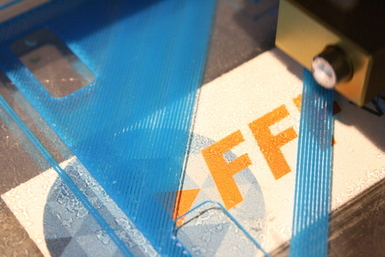
\includegraphics[width=\textwidth,cfbox=azul_marcos 3pt 0pt]{FOTOS/HOTENDALTO}
	\caption*{Nozzle too far}
    \end{subfigure}
    ~ %add desired spacing between images, e. g. ~, \quad, \qquad, \hfill etc. 
      %(or a blank line to force the subfigure onto a new line)
    \begin{subfigure}[b]{0.3\textwidth}
        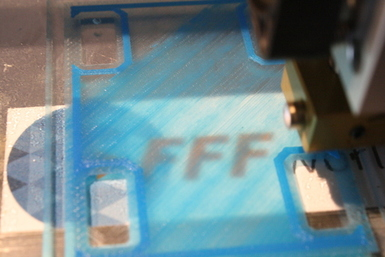
\includegraphics[width=\textwidth,cfbox=azul_marcos 3pt 0pt]{FOTOS/HOTENDBAJO}
	\caption*{Nozzle too close}
    \end{subfigure}
    ~ %add desired spacing between images, e. g. ~, \quad, \qquad, \hfill etc. 
    %(or a blank line to force the subfigure onto a new line)
    \begin{subfigure}[b]{0.3\textwidth}
        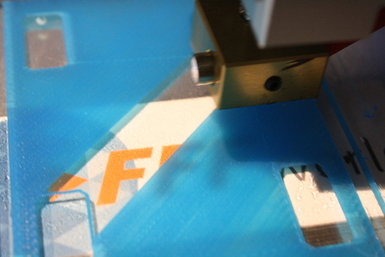
\includegraphics[width=\textwidth,cfbox=azul_marcos 3pt 0pt]{FOTOS/HOTENDPERFECTO}
	\caption*{Nozzle well leveled}
    \end{subfigure}
\end{figure}
Questa regolazione può essere effettuata attraverso il software, regolando il z-offset nel programma di laminazione, o regolando il meccanismo di livellazione della piattaforma di stampa.
	\subsection{Consigli di laminazione}
		\subsubsection{L'altezza dello strato}
L'altezza dello strato determina la qualità del pezzo e il tempo di stampa.
\\\\
Utilizzando un nozzle da 0.4 mm abbiamo notato che l'altezza ottimale dello strato è di 0.2 mm. Con questa altezza si otterranno strati fortemente uniti con una finitura della superficie eccellente.
		\subsubsection{I top layers e perimetri}
I top layers e i perimetri sono la copertura laterale e superiore del pezzo. Il numero adeguato di questi dipenderà dall'infill e dall'uso che si andrà a fare del pezzo.
\\\\
Con un infill alto si può ridurre il numero di top-layers a 3, dato che la parte piena del pezzo darà loro una buona base dove appoggiarsi. Utilizzando dei valori di infill medi o bassi è consigliabile aumentare il numero di top-layers a 5, per essere sicuri che la parte superiore del pezzo sia completamente sigillata.
\\\\
Se il pezzo deve subire deformazioni è consigliabile aumentare il numero di shells o perimetri orizzontali. Aumentando il numero di perimetri orizzontali si eviterà che nelle pareti del pezzo possano crearsi fessure se si effettua pressione o trazione su di esse. 
\\\\
Questi consigli sono validi quando si usa un nozzle da 0.4 mm e un'altezza di strato di 0.2 mm. Se la dimensione del nozzle o l'altezza dello strato variano, anche il numero di perimetri e di top-layers ottimali cambierà
\\\\
Ti invitiamo ad effettuare le tue prove e a condividere con noi il risultato. 
		\subsubsection{Influenza dell'infill nella flessibilità}
La quantità e il disegno dell'infill ha una grande influenza nel grado di flessibilità dei pezzi stampati con FlexiSMART.
\\\\
Un pezzo con un infill vicino al 100\% si comporterà come un blocco di gomma e può essere una buona opzione per pezzi come silent-blocks o spacers.
\\\\
Utilizzando un infill del 15\% si otterranno pezzi molli che potranno essere schiacciati e deformati.
\\\\
Anche il modello di infill condiziona la flessibilità, non hanno lo stesso comportamento un infill rettilineo e uno honeycomb (a nido d'ape). Ti consigliamo di effettuare le tue prove e scegliere quello più adatto al tuo progetto.
	\subsection{Utilizzo di un nozzle di dimensioni maggiori }
La maggior parte delle stampanti utilizza di serie un nozzle da 0.4 mm, una dimensione di nozzle che offre una buona proporzione velocità/risoluzione. FlexiSMART si stampa perfettamente con questo tipo di nozzle, comunque è bene fare una puntualizzazione.
\\\\
La dimensione del nozzle limita la quantità di materiale che può essere estruso per unità di tempo. Utilizzando filamenti rigidi questo limite è maggiore, dato che si può aumentare la velocità e il filamento sopporta la pressione extra necessaria affinché il materiale esca dal nozzle. Con FlexiSMART, tuttavia, il filamento si comprime se questa pressione è troppo alta e, generalmente, deve essere stampato a velocità minore. 
\\\\
Perciò, se vuoi estruire FlexiSMART a velocità elevate, è consigliabile l'utilizzo di un nozzle di dimensioni maggiori, a partire da 0.6 mm. Utilizzando uno di questi nozzle potrai stampare molto più rapidamente, con altezze degli strati superiori, sacrificando qualcosa nella risoluzione. 
\section{Desideri supportare il nostro progetto?}
Tutti i membri FFF World amano la stampa 3D e la comunità maker. Ci consideriamo fortunati di poter lavorare a progetti nei quali possiamo mettere la nostra sincera passione. Nel futuro, ci piacerebbe poter sviluppare più materiali, più colori e più formati. Insomma, ci piacerebbe poter far crescere la nostra impresa.
\\\\
Per poterlo fare, una delle principali azioni per aiutarci, se desideri farlo e se sei soddisfatto del filamento, è quella di lasciarci un feedback da 5 stelle su Amazon.
\begin{figure}[H]
\centering

\includegraphics[width=0.5\textwidth,cfbox=azul_marcos 1pt 0pt]{FOTOS/AMAZON_FIVE_STARS}
\caption*{Grazie mille!}
\end{figure}
\subsection{Altri materiali con fantastiche proprietà disponibili su Amazon}
\begin{description}
\item[FlexiSMART Tech:] Progettato per resistere all'abrasione e al logorio di stampe tecniche.
\item[ABS Tech:] Effetto warping minimizzato. Alto rendimento in applicazioni tecniche.
\item[PETG Tech:] Massima resistenza meccanica. Resistente al contatto con l'acqua e ai raggi UV. Adatto per uso alimentare. 
\item[FilaMETAL:] PLA con carica metallica non abrasiva che fornisce una finitura metallica spettacolare alle tue stampe. 
\item[PC Tech:] Policarbonato ad alta resistenza alla temperatura e con eccellenti proprietà meccaniche.
\item[Nylon Tech:] Stampabile a bassa temperatura. Resistenza ai colpi con un certo grado di flessibilità.
\item[PVA Tech:] Filamento solubile in acqua indicato per essere utilizzato come materiale di supporto. Eccellente compatibilità con PLA.
\item[HIPS Tech:] Filamento solubile in limonene indicato per essere utilizzato come materiale di supporto. Buona resistenza meccanica ed eccellente compatibilità con ABS.
\end{description}
%\section{Bibliografía}
%Esta guía no habría sido posible sin el conocimiento libre generado por la comunidad RepRap. Para la elaboración de esta guía se han %utilizado imágenes y contenido extraidos de los siguientes sitios web.
%\\\\
%\url{http://www.gyrobot.co.uk/blog/how-to-3d-print-with-flexible-filaments}\\
%\url{http://www.thingiverse.com/thing:1496895}\\
%\url{http://www.thingiverse.com/thing:247024}\\
%\url{http://www.thingiverse.com/thing:16319}\\
%\url{http://www.thingiverse.com/thing:779011}\\
%\url{http://www.thingiverse.com/thing:1102900}\\
%\url{http://www.thingiverse.com/thing:147705}\\
%\url{http://www.thingiverse.com/thing:222667}\\
%\url{http://www.thingiverse.com/thing:512338}\\
%\url{https://all3dp.com/common-3d-printing-problems-and-their-solutions/}\\
%\url{https://www.simplify3d.com/support/}\\
%\url{http://www.thingiverse.com/thing:508896}\\
%\url{http://www.thingiverse.com/thing:1187344}

\includepdf{PDF/IT_CONTRAPORTADA.pdf}
\end{document}
